\section{Results}
%---------------------------------------------------------------------------------------------------
\subsection{Risk Group Duration}\label{res.yss}
% compare FSW duration after each stage of adjustment
Figure~\ref{fig:yss.adj}
\begin{figure}
  \centering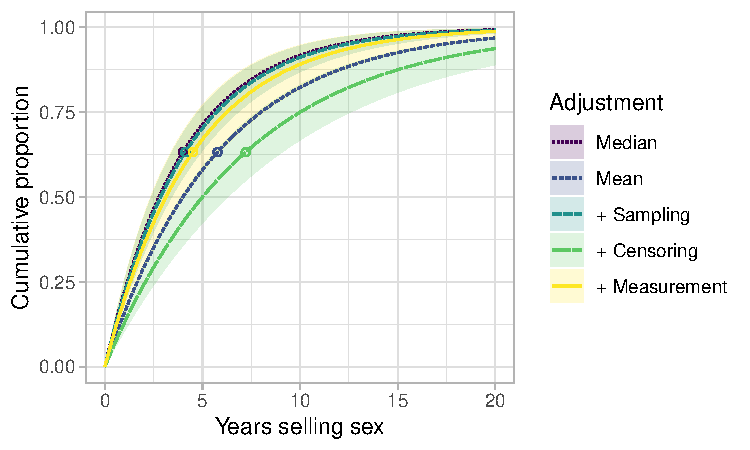
\includegraphics[scale=.75]{yss.adj}
  \caption{TODO}
  \label{fig:yss.adj}
\end{figure}
%---------------------------------------------------------------------------------------------------
\subsection{Sexual Partnership Duration}\label{res.partners}
% infer adjusted partnership Q, K & compare to naive estimates
\begin{figure}[h]
  \centering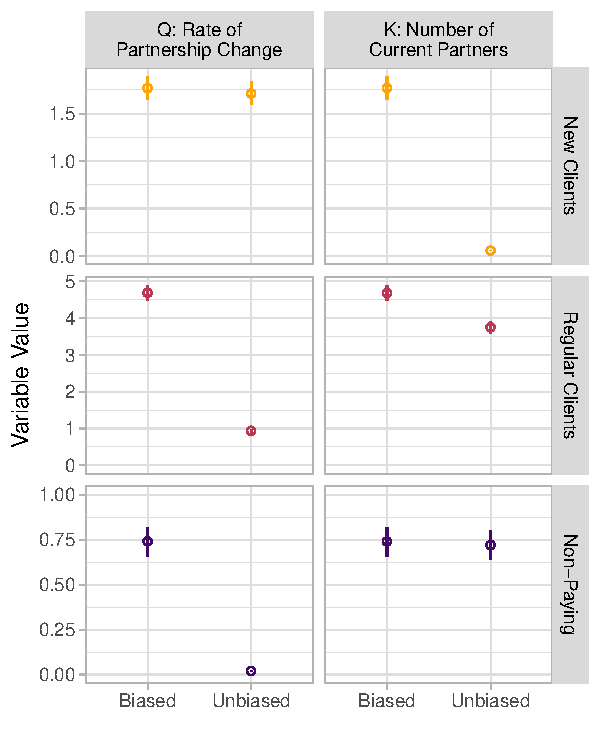
\includegraphics[scale=.8]{partners.fsw}
  \caption{Biased vs unbiased estimates of:
    number of current partners and rate of partnership change,
    for three partnership types reported by female sex workers in \cite{Baral2014}.
    Error bars show 95\%~CI from 10,000 simulated surveys with $N = 328$.}
  \label{fig:partners.fsw}
\end{figure}
\begin{figure}[h]
  \centering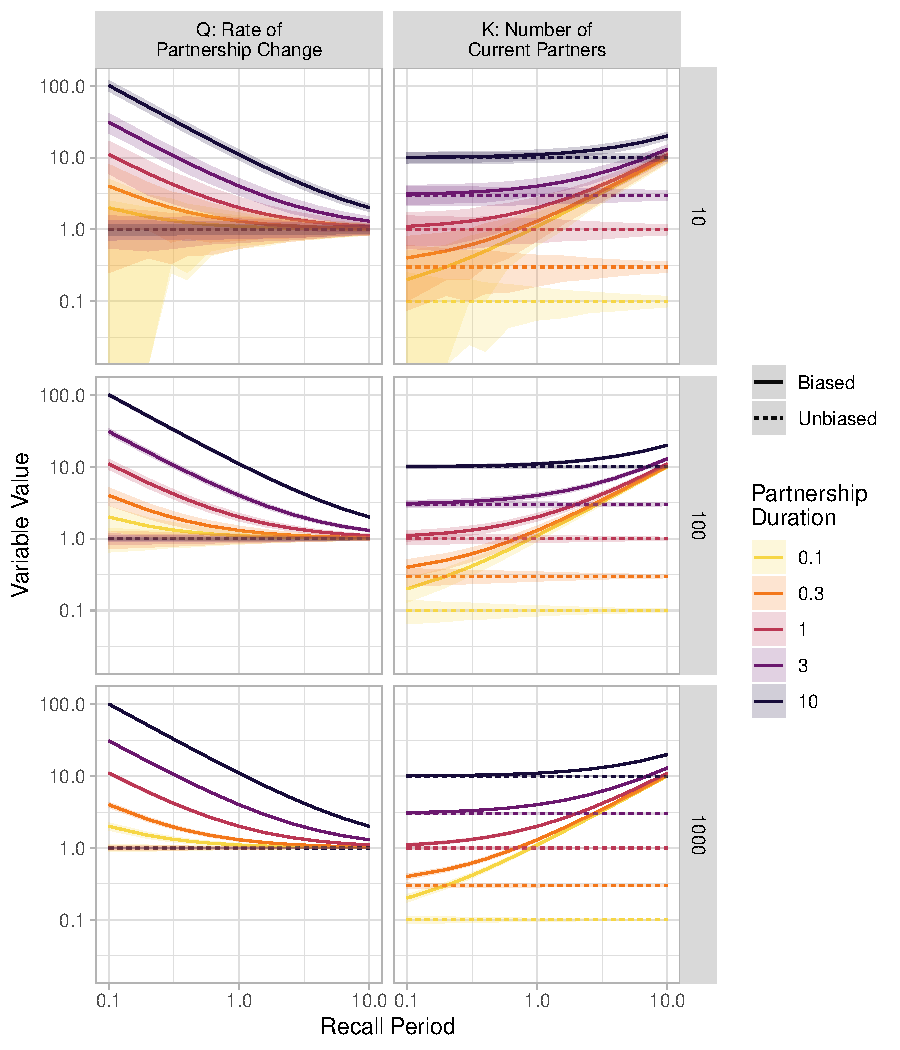
\includegraphics[scale=.8]{partners.sens}
  \caption{Biased vs unbiased estimates of:
    number of current partners and rate of partnership change,
    for different recall periods and partnership durations.
    Ribbons show 95\%~CI from 10,000 simulated surveys with $N = 10, 100, 1000$.}
  \label{fig:partners.sens}
\end{figure}
